% 独自のコマンド

% ■ アブストラクト
%  \begin{jabstract} 〜 \end{jabstract}  :日本語のアブストラクト
%  \begin{eabstract} 〜 \end{eabstract}  :英語のアブストラクト

% ■ 謝辞
%  \begin{acknowledgment} 〜 \end{acknowledgment}

% ■ 文献リスト
%  \begin{bib}[100] 〜 \end{bib}


\newif\ifjapanese

\japanesetrue  % 論文全体を日本語で書く(英語で書くならコメントアウト)

\ifjapanese
  %\documentclass[a4j,twoside,openright,11pt]{jreport} % 両面印刷の場合。余白を綴じ側に作って右起こし。
  \documentclass[a4j,11pt]{jreport}                  % 片面印刷の場合。
  \renewcommand{\bibname}{参考文献}
  \newcommand{\acknowledgmentname}{謝辞}
\else
  \documentclass[a4paper,11pt]{report}
  \newcommand{\acknowledgmentname}{Acknowledgment}
\fi
\usepackage{thesis}
\usepackage{ascmac}
\usepackage{graphicx}
\usepackage{multirow}
\usepackage{url}
\usepackage{listings,jlisting}
\bibliographystyle{jplain}

%\bindermode  % バインダー用余白設定

% 日本語情報(必要なら)
\jclass  {卒業プロジェクト}                             % 論文種別
%\jtitle    {汎用的なAndroid Widgetの作成及び\\それを用いた情報獲得手法の提案}    % タイトル。改行する場合は\\を入れる
\jtitle    {リアルタイム情報の効率的閲覧システムの研究}    % タイトル。改行する場合は\\を入れる
\juniv    {慶應義塾大学}                  % 大学名
\jfaculty  {環境情報学部}               % 学部、学科
\jauthor  {中山 拓哉}                       % 著者
\jhyear  {26}                                   % 平成○年度
\jsyear  {2014}                                 % 西暦○年度
\jkeyword  {Linda、Android、Android Widget}     % 論文のキーワード
\jproject{増井俊之研究会} %プロジェクト名
\jdate{2015年1月}


\begin{document}

\ifjapanese
  \jmaketitle    % 表紙(日本語)
\else
  \emaketitle    % 表紙(英語)
\fi

% ■ アブストラクトの出力 ■
%	◆書式:
%		begin{jabstract}〜end{jabstract}	:日本語のアブストラクト
%		begin{eabstract}〜end{eabstract}	:英語のアブストラクト
%		※ 不要ならばコマンドごと消せば出力されない。



% 日本語のアブストラクト
\begin{jabstract}
スマートフォンの普及によって天気や電車の運行情報などを取得することは容易になったが、それぞれの情報にアクセスするためには専用のアプリケーションを使用する必要がある。

汎用的なAndroid Widgetを用いることで専用のアプリケーションを用いること無く複数の種類の情報を取得する事が出来るようになる。

\end{jabstract}



% 英語のアブストラクト
  % アブストラクト。要独自コマンド、include先参照のこと

\tableofcontents  % 目次
\listoffigures    % 表目次
\listoftables    % 図目次

\pagenumbering{arabic}

\chapter{序論}
\label{chap:introduction}
\section{背景}

% なぜこの研究が必要だったのか、しっかりした理屈を考えておく。
% 現状どういう問題があるのか
% どういう方法で解決を試みたのか
% 結果として上手く行ったのか、いかなかったのか

近年、スマートフォンなどのモバイルインターネット端末は爆発的に普及し、利用者の年代を問わず用いられるようになった。
生活の一部とも言える存在となったこれらの端末だが、私がこれらの端末を使用する中で不便だと感じる点がある。
それは取得したいと思う情報を思うように得られないという点である。スマートフォンを用いて情報を獲得する手法としてAndroid Widgetは普遍的に用いられている。
天気予報を見たければ天気予報のWidgetを画面に設置し、別の情報が必要であればまた別のWidgetを設置する。
設置してさえおけばユーザーが能動的に操作をしなくとも最新の情報を常に画面に表示してくれるので情報の獲得手法としては有能である。

しかし、Android Widgetは多くの問題点も抱えている。
まずAndroid端末の一つの画面に置くことの出来るWidgetの数は限られているため獲得できる情報の種類も限られてしまうという問題である。(図\ref{fig:old_widget})
しかもAndroid Widgetの性質上取得したい情報に付随して不要な情報までもが表示され、それによって画面スペースを埋められてしまうといったケースも存在する。
また、自分の取得したい情報に対応したWidgetが存在しない場合、自らWidgetを作成するしか無いといった問題もある。
現状ではAndroid Widgetの作成は技術的なハードルが高く問題の解決法としては現実的ではない。

そこで私はあらゆる情報に対応した汎用的なAndroid Widgetを作成することでこれらの状況を解決したいと考えた。

\begin{figure}[htbp]
  \begin{minipage}{\hsize}
    \begin{center}
      \fbox{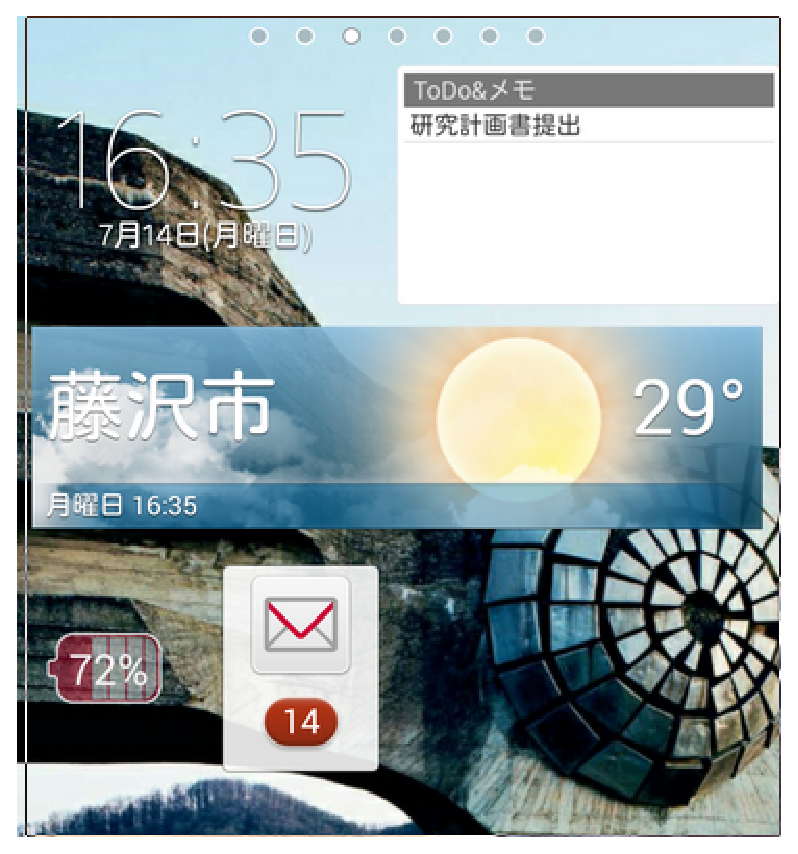
\includegraphics[width=80mm]{image/old_widget.eps}}
    \end{center}
    \caption{現状のWidgetの使用した画面}
    \label{fig:old_widget}
  \end{minipage}
\end{figure}

\section{目的}
あらゆる情報を容易に獲得するための手法を提案・作成する。まずはユーザーが必要とする可能性のある情報を予め取得し、記録しておくことが必要である。次に記録したデータからユーザーが求めるもののみを選択しユーザーに提供することでユーザーが取得したい情報のみをいつでも取得できている状況を作り出す。

\section{本論文の構成}
第\ref{chap:introduction}章では本研究の概要を書いた。

第\ref{chap:contents}章では研究内容を説明する。第\ref{chap:prototype}章ではプロトタイプの実装方法を解説する。第\ref{chap:consideration}章では考察を書く。最後に第\ref{chap:conclusion}章にて結論を書き本論文をしめることとする。添付として参考文献を追記する。
  % 本文1
\chapter{研究内容}
\label{chap:contents}

本章では、本研究の内容を説明する。

\section{システム概要}

本システムの目的はユーザーが必要とする複数の情報を提供することで、ユーザーが効率良く価値の高い情報を得られるようにすることである。

以下にシステムの構成を示す。

\begin{table}[htbp]
  \caption{システム構成}
  \label{tb:files}
  \begin{center}\begin{tabular}{|c|p{12cm}|}
    \hline
    システム&概要\\\hline\hline
    {\tt Linda}&データ元。データストリームからデータを取得する。\\\hline
    {\tt サーバー}&Androidクライアントからのリクエストがに応じLindaからデータを取得しAndroidクライアントに送信する。外部から取得したデータをLindaに書き込む。\\\hline
    {\tt WEBクライアント}&Androidクライアントに送信する情報を選択する為のビューを提供する。\\\hline
    {\tt Androidクライアント}&サーバーにデータを要求し、ユーザーに情報を表示する。\\\hline
    {\tt データベース}&サーバーのデータを保存している。\\\hline
  \end{tabular}\end{center}
\end{table}

サーバーは各種APIなどを用いてユーザーが必要とする情報を取得しLinda\footnote{http://linda.masuilab.org/\\データをクラウド上で共有するためのフレームワーク。並列処理で同時に多くのクライアントを処理できる。}へと書き込み、Androidクライアントからのリクエストに応じてLindaからデータを取得しJSON形式でレスポンスを返す。
Androidクライアントはユーザーの操作に応じてサーバーにリクエストを送り、サーバーから返されたJSONをパースして表示する。

\subsection{データの取得と記録}
データの取得方法は三つ存在する。

まず一つ目として既存のAPIを用いて取得する方法である。天気予報や株価の情報など比較的ポピュラーな情報であれば既にAPIが存在するので、それらを用いて定期的にサーバーがデータを取得しLindaへ書き込む。(図\ref{fig:weather_widget})の例ではYQL\footnote{Yahoo query language}を用いて取得した天気予報をAndroid Widgetとして表示している。

二つ目はAPIが存在しないWebページ上の情報である。例として自分の利用する公共交通機関の運行情報や特定の商品の在庫情報などである。これらのデータはKimono\footnote{https://www.kimonolabs.com/\\指定したWebページをスクレイピングし、API化するサービス。}を用いて取得したい部分に対応するAPIを作成しデータを取得する。(図\ref{fig:odakyu_widget})の例では小田急電鉄のWebページ\footnote{http://www.odakyu.jp/cgi-bin/user/emg/emergency\_bbs.pl}(図\ref{fig:odakyu_page})にて公開されている列車の運行情報をKimonoを用いてAPI化して取得し、Android Widgetとして表示している。

三つ目はセンシングデータである。自室などに設置した各種センサーからのデータに関してはセンシングする機器から直接Lindaに書き込むか、もしくはセンシングする機器からサーバー経由でLindaに書き込む。(図\ref{fig:sensor_widget})の例ではArduinoと明るさセンサー、温度センサーを用いてLindaにそれぞれの値を書き込こむ為の機構である。

\begin{figure}[htbp]
  \begin{minipage}{\hsize}
    \begin{center}
      \fbox{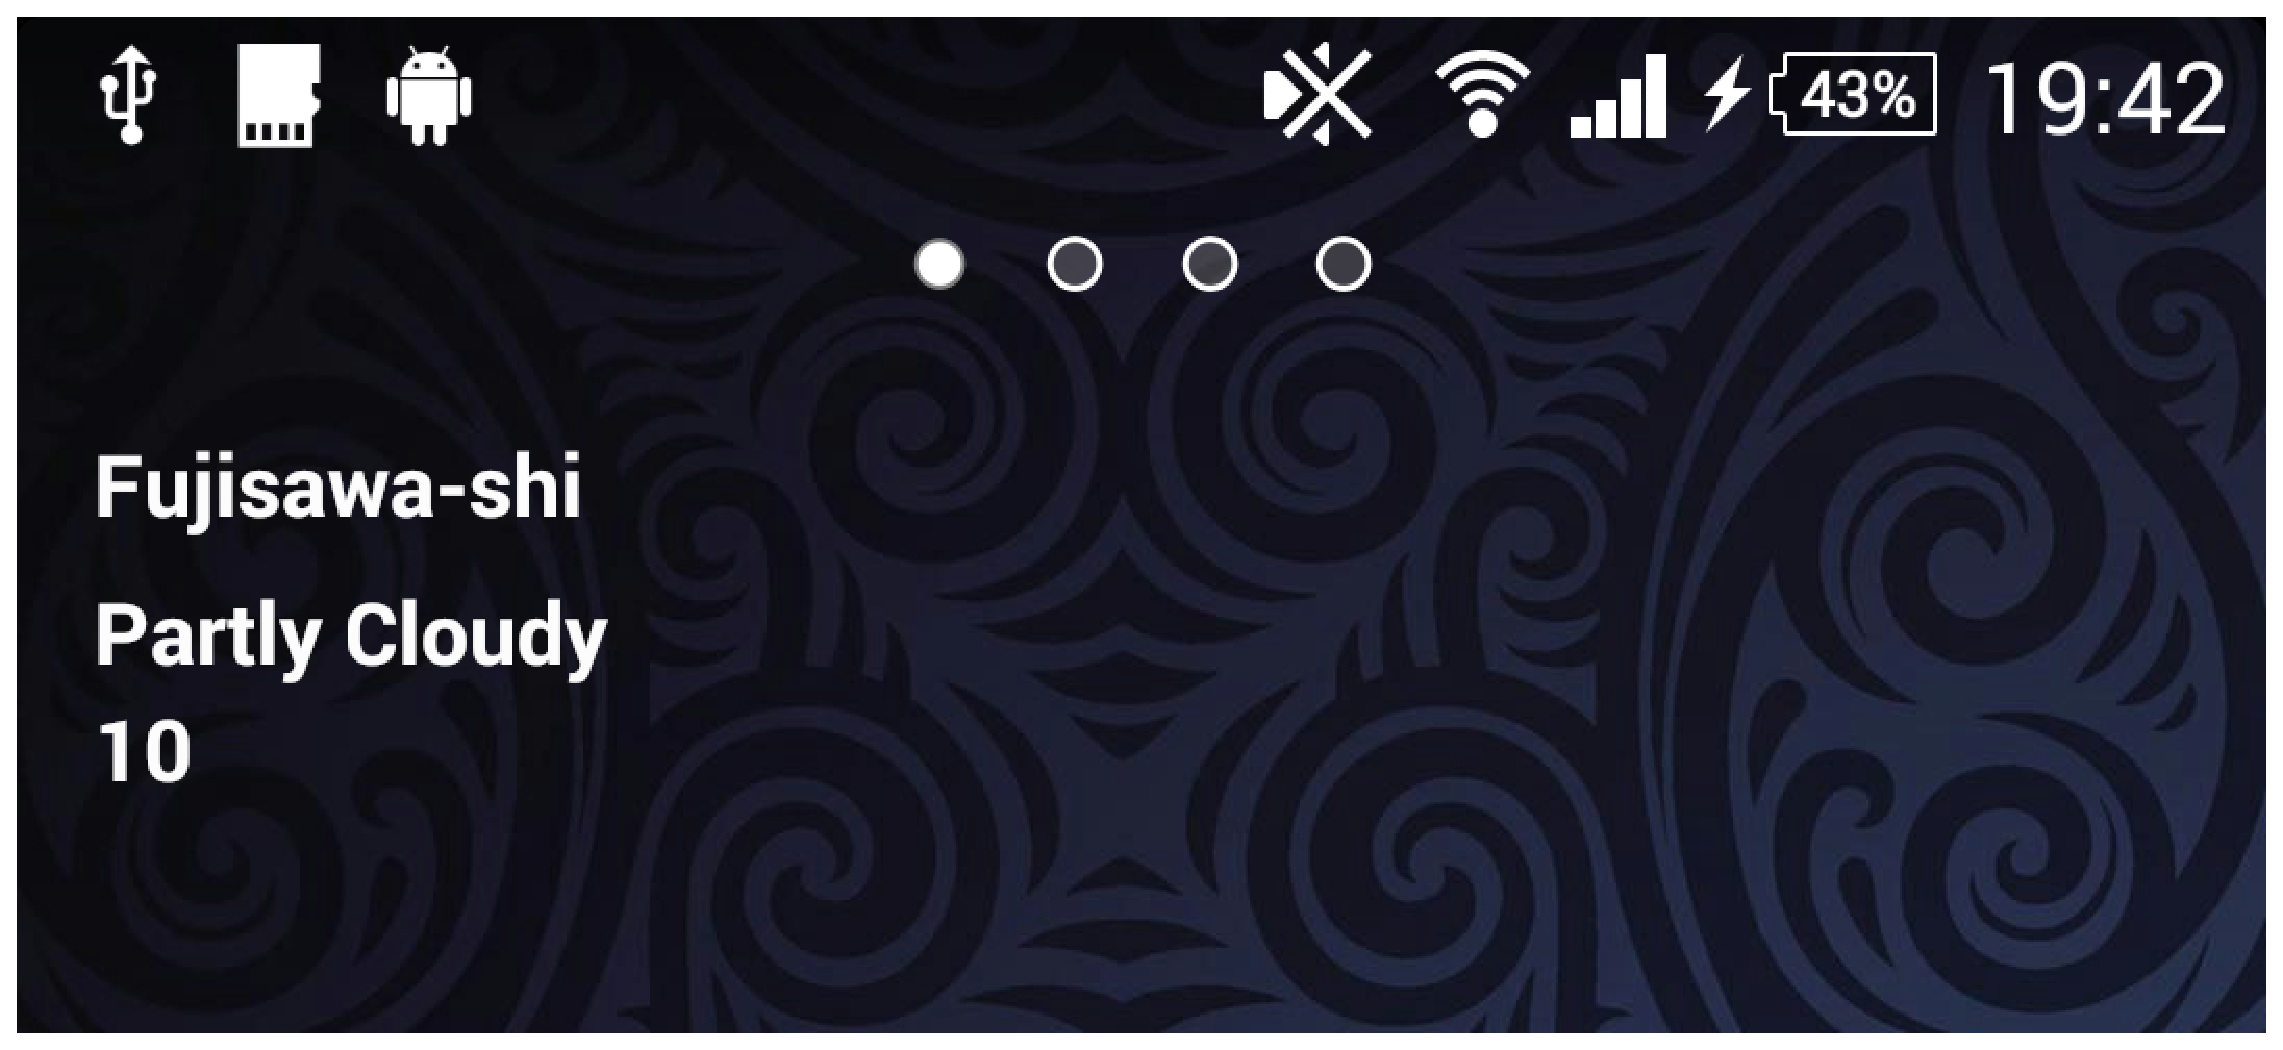
\includegraphics[width=100mm]{image/weather_widget.eps}}
    \end{center}
    \caption{天気予報をAndoid Widgetとして表示}
    \label{fig:weather_widget}
  \end{minipage}
\end{figure}

\begin{figure}[htbp]
  \begin{minipage}{\hsize}
    \begin{center}
      \fbox{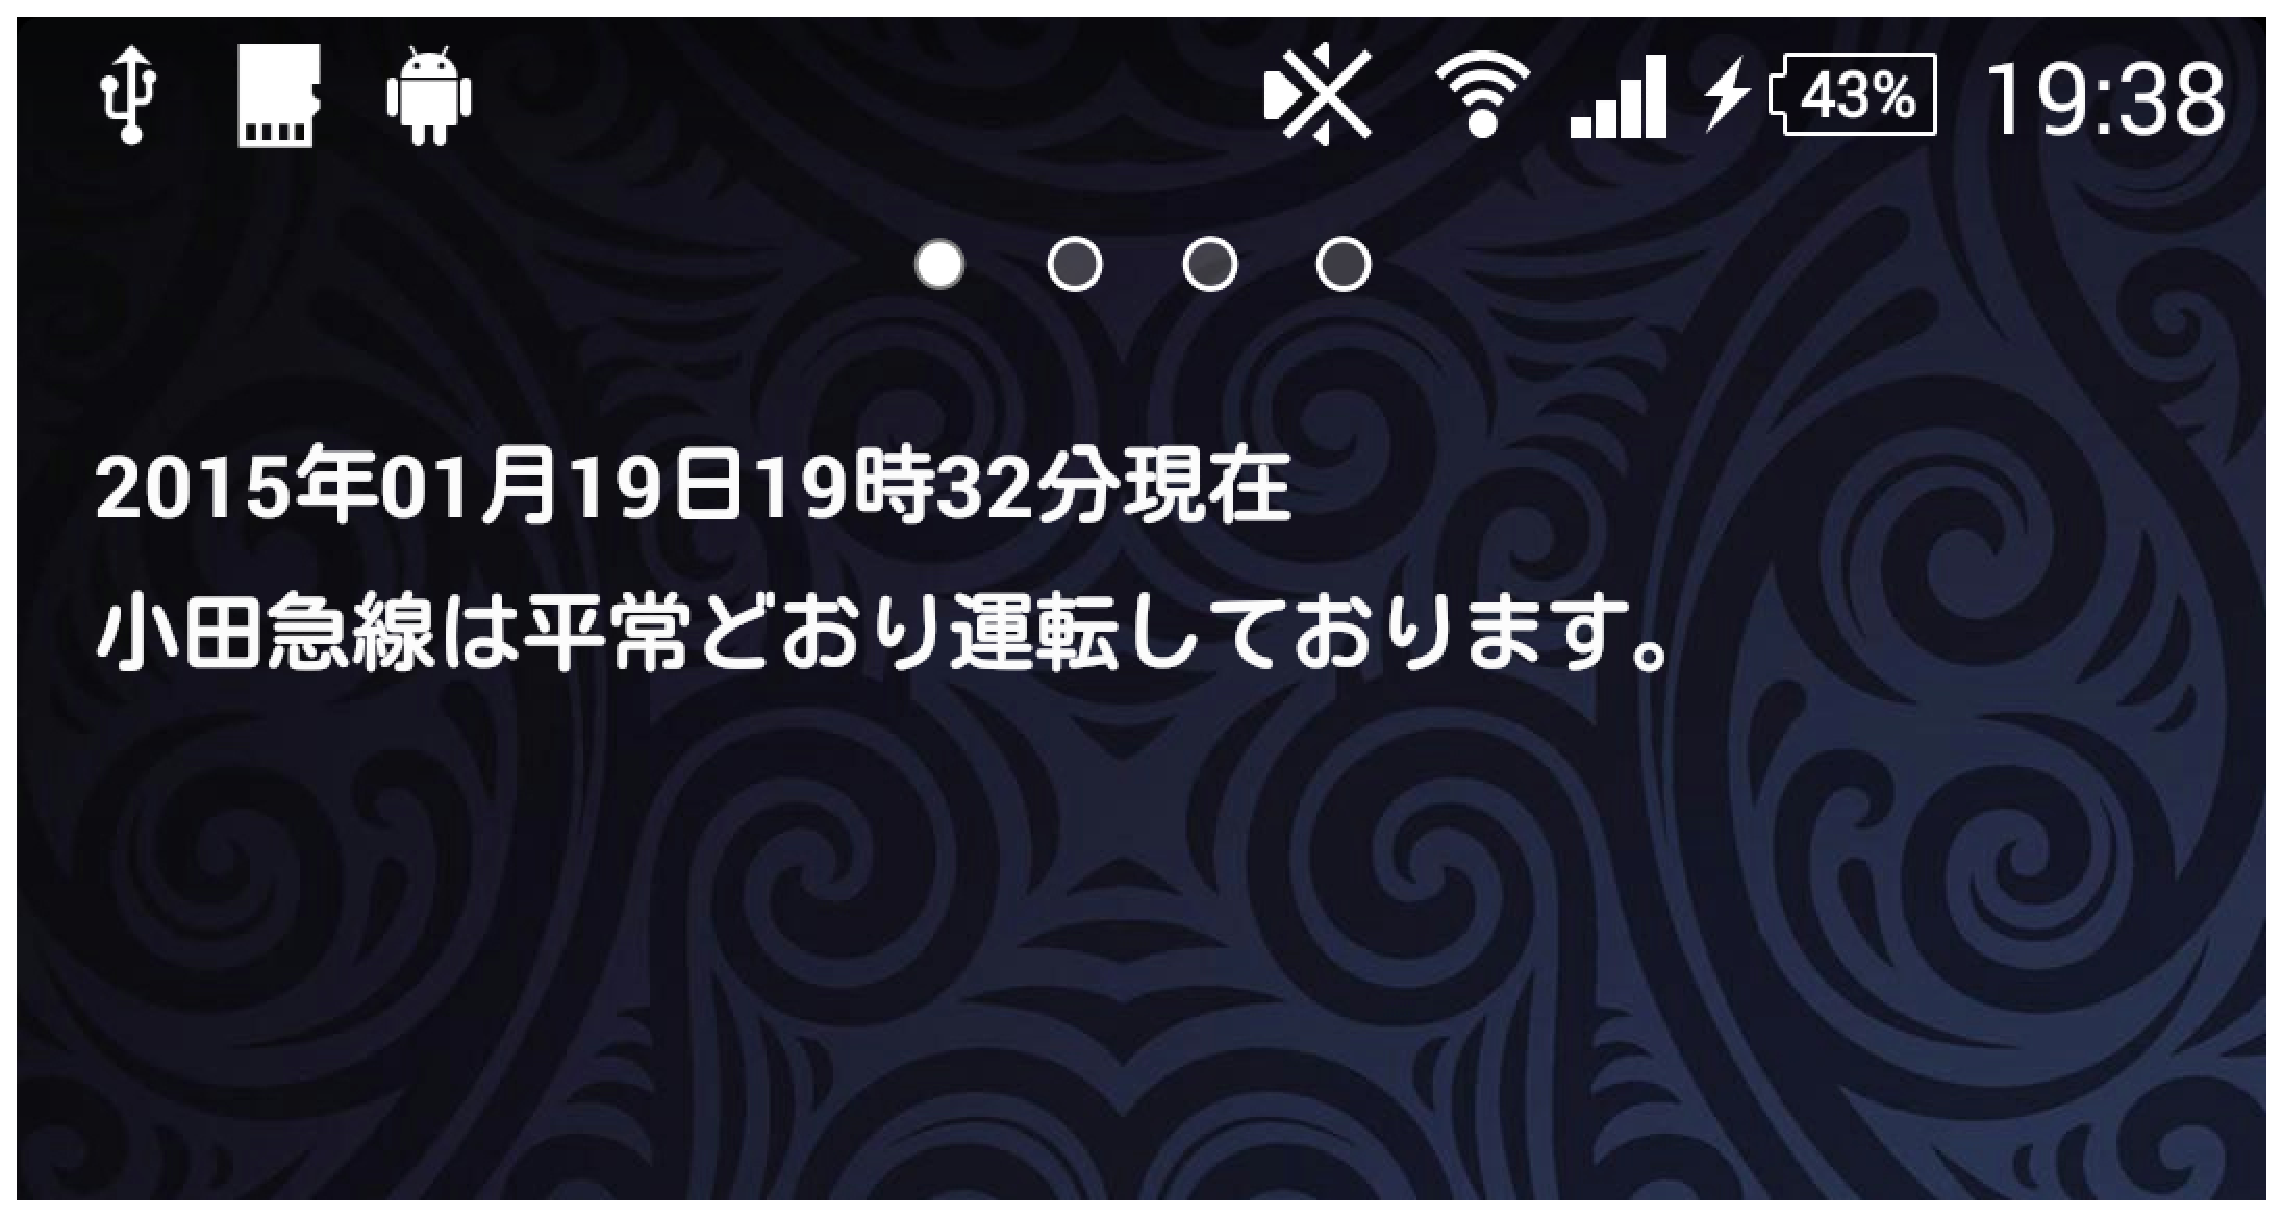
\includegraphics[width=100mm]{image/odakyu_widget.eps}}
    \end{center}
    \caption{小田急電鉄の運行情報を表示}
    \label{fig:odakyu_widget}
  \end{minipage}
\end{figure}

\begin{figure}[htbp]
  \begin{minipage}{\hsize}
    \begin{center}
      \fbox{
\includegraphics[width=100mm]{image/odakyu.eps}}
    \end{center}
    \caption{小田急電鉄の運行情報を公開しているWebページ}
    \label{fig:odakyu_page}
  \end{minipage}
\end{figure}

\begin{figure}[htbp]
  \begin{minipage}{\hsize}
    \begin{center}
      \fbox{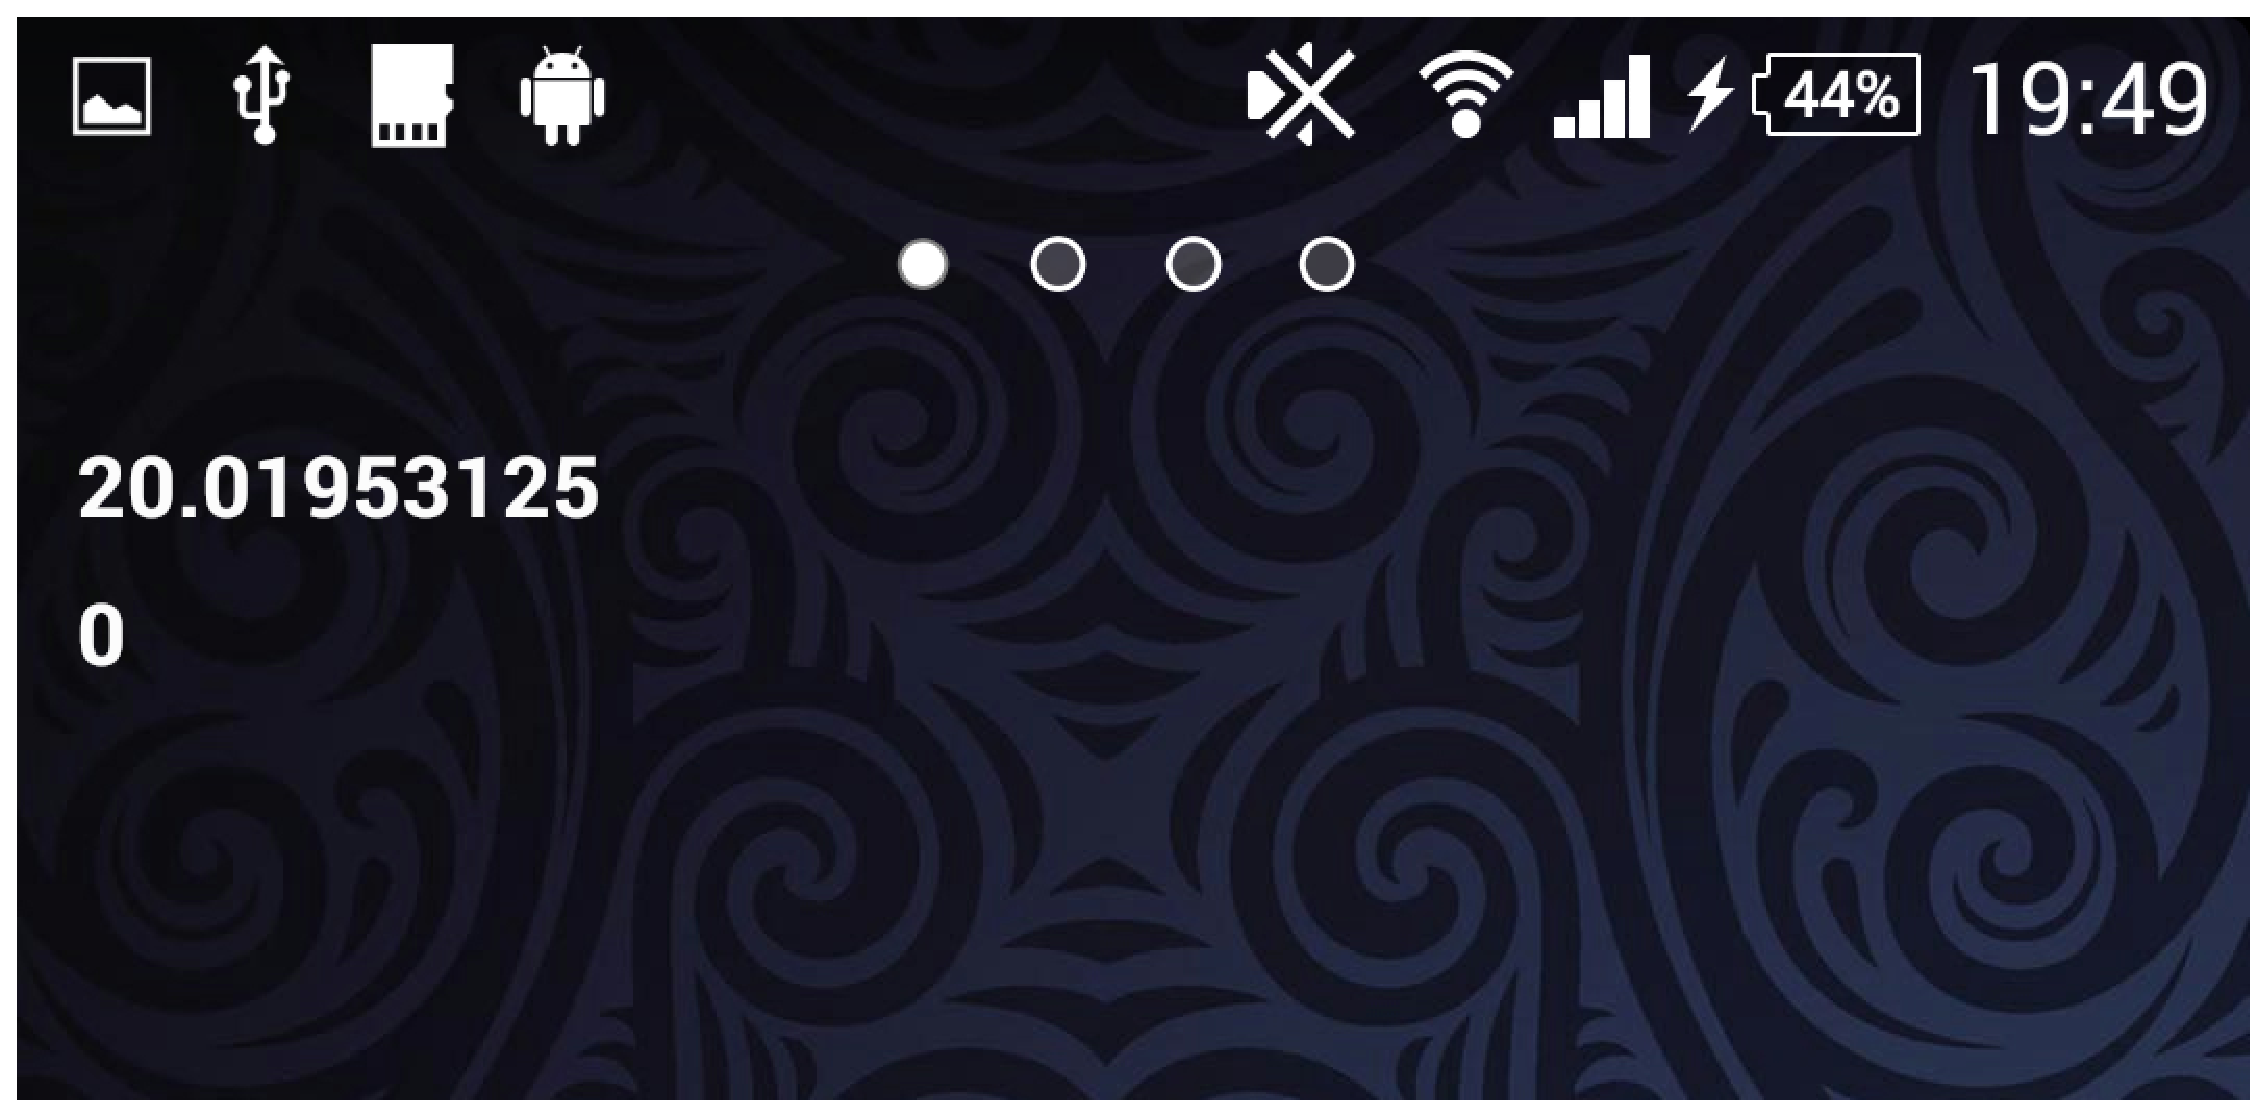
\includegraphics[width=100mm]{image/sensor_widget.eps}}
    \end{center}
    \caption{センサーデータをWidgetとして表示}
    \label{fig:sensor_widget}
  \end{minipage}
\end{figure}

\begin{figure}[htbp]
  \begin{minipage}{\hsize}
    \begin{center}
      \fbox{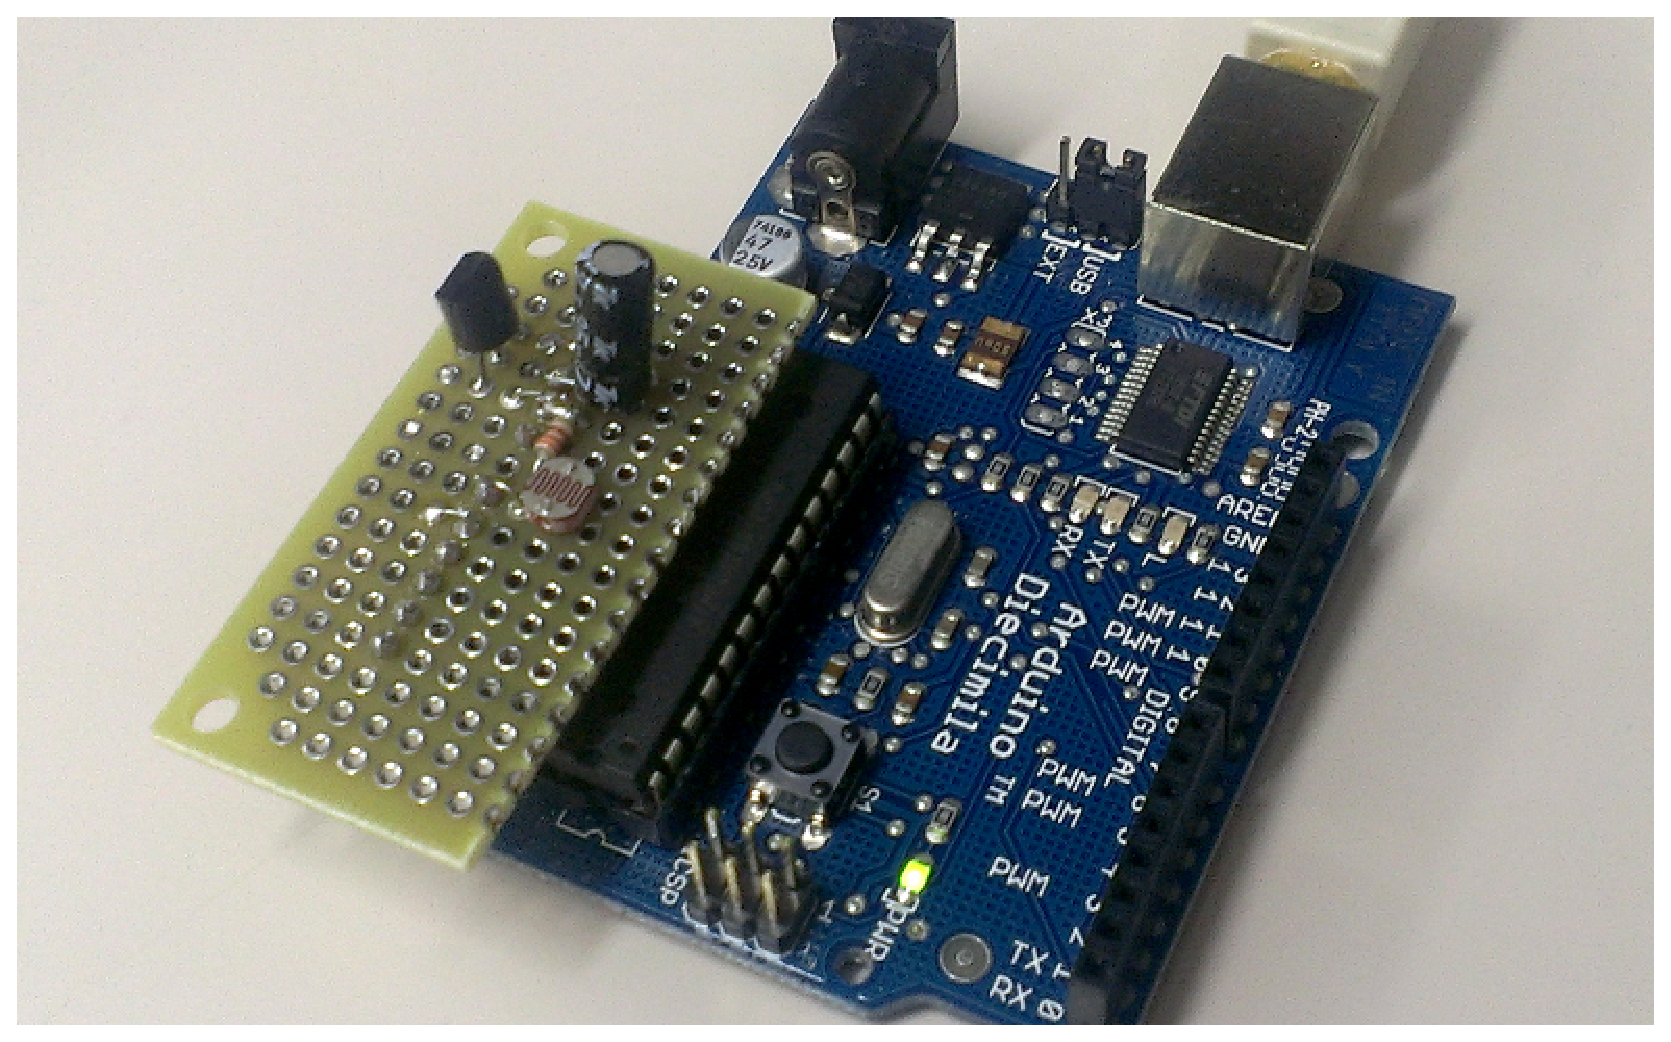
\includegraphics[width=100mm]{image/arduino_sensor.eps}}
    \end{center}
    \caption{明るさと温度を取得するセンサーとArduino}
    \label{fig:arduino_sensor}
  \end{minipage}
\end{figure}

\subsection{ユーザーが受け取るデータの選択}

ユーザーは受け取りたい情報をWebページ上から指定する。Lindaサーバーに存在するデータの中から受け取りたい情報に対応したTupleTypeとTupleNameのペアを指定する。(図\ref{fig:select})このペアはデータベースに保存され、JSONを生成する際に参照される。

\begin{figure}[htbp]
  \begin{minipage}{\hsize}
    \begin{center}
      \fbox{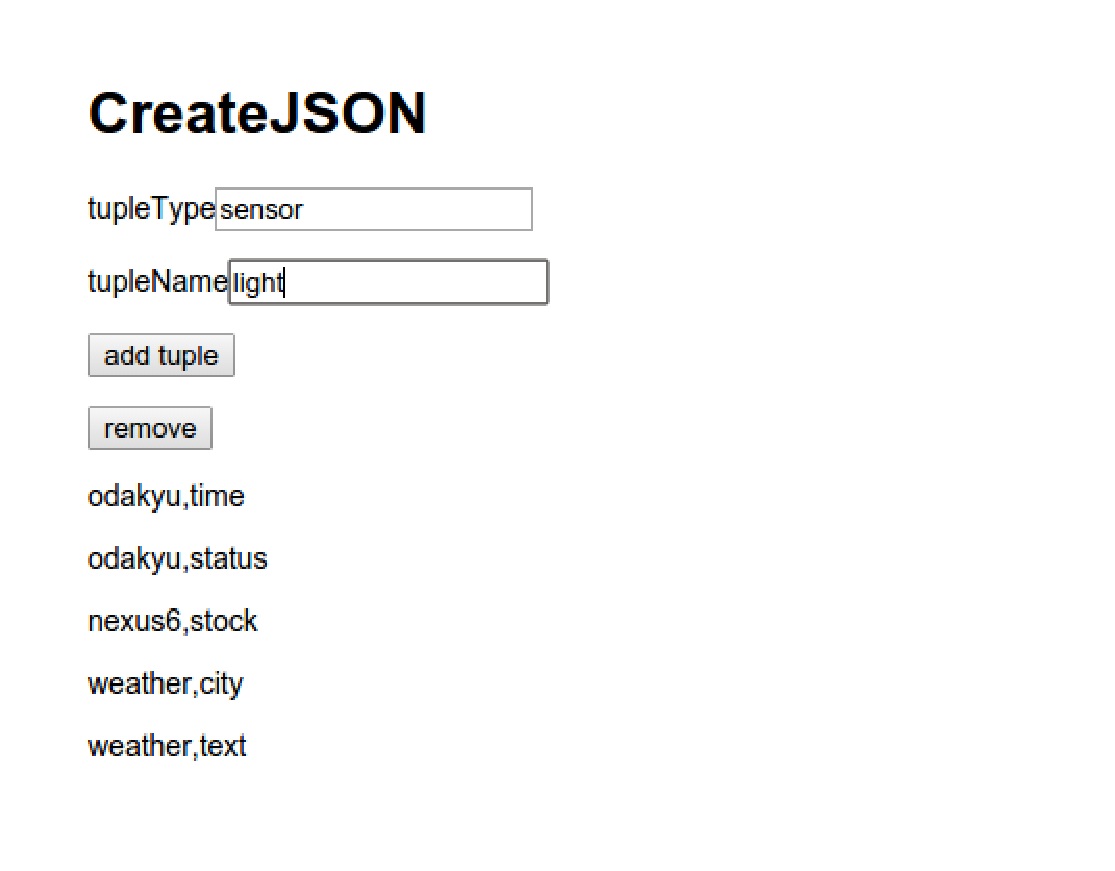
\includegraphics[width=100mm]{image/select.eps}}
    \end{center}
    \caption{Androidクライアントに送信するデータの選択画面}
    \label{fig:select}
  \end{minipage}
\end{figure}

\subsection{ユーザーへの情報の提供}
ユーザーが選択した情報はサーバーによって取得されJSON形式でAndroid端末へと送られる。(図\ref{fig:JSON})Androidは受け取ったJSONをパースしAndroid Widgetとして表示する。(図\ref{fig:widget})

サーバーへのリクエストは15分間隔のAndroid Widgetの自動更新の際と、ユーザーがAndroid Widgetをタップした際に実行される。

\begin{figure}[htbp]
  \begin{minipage}{\hsize}
    \begin{center}
      \begin{lstlisting}[basicstyle=\ttfamily\footnotesize, frame=single]

      {
          "info": [
              {
                  "0": "2015年01月16日14時43分現在",
                  "1": "小田急線は平常どおり運転しております。",
                  "2": "We are out of inventory. Please check back soon.",
                  "3": "Fujisawa-shi",
                  "4": "Mostly Cloudy"
              }
          ]
      }

      \end{lstlisting}
    \end{center}
    \caption{サーバーから送られるJSONの例}
    \label{fig:JSON}
  \end{minipage}
%\end{figure}

%\begin{figure}[htbp]
  \begin{minipage}{\hsize}
    \begin{center}
      \fbox{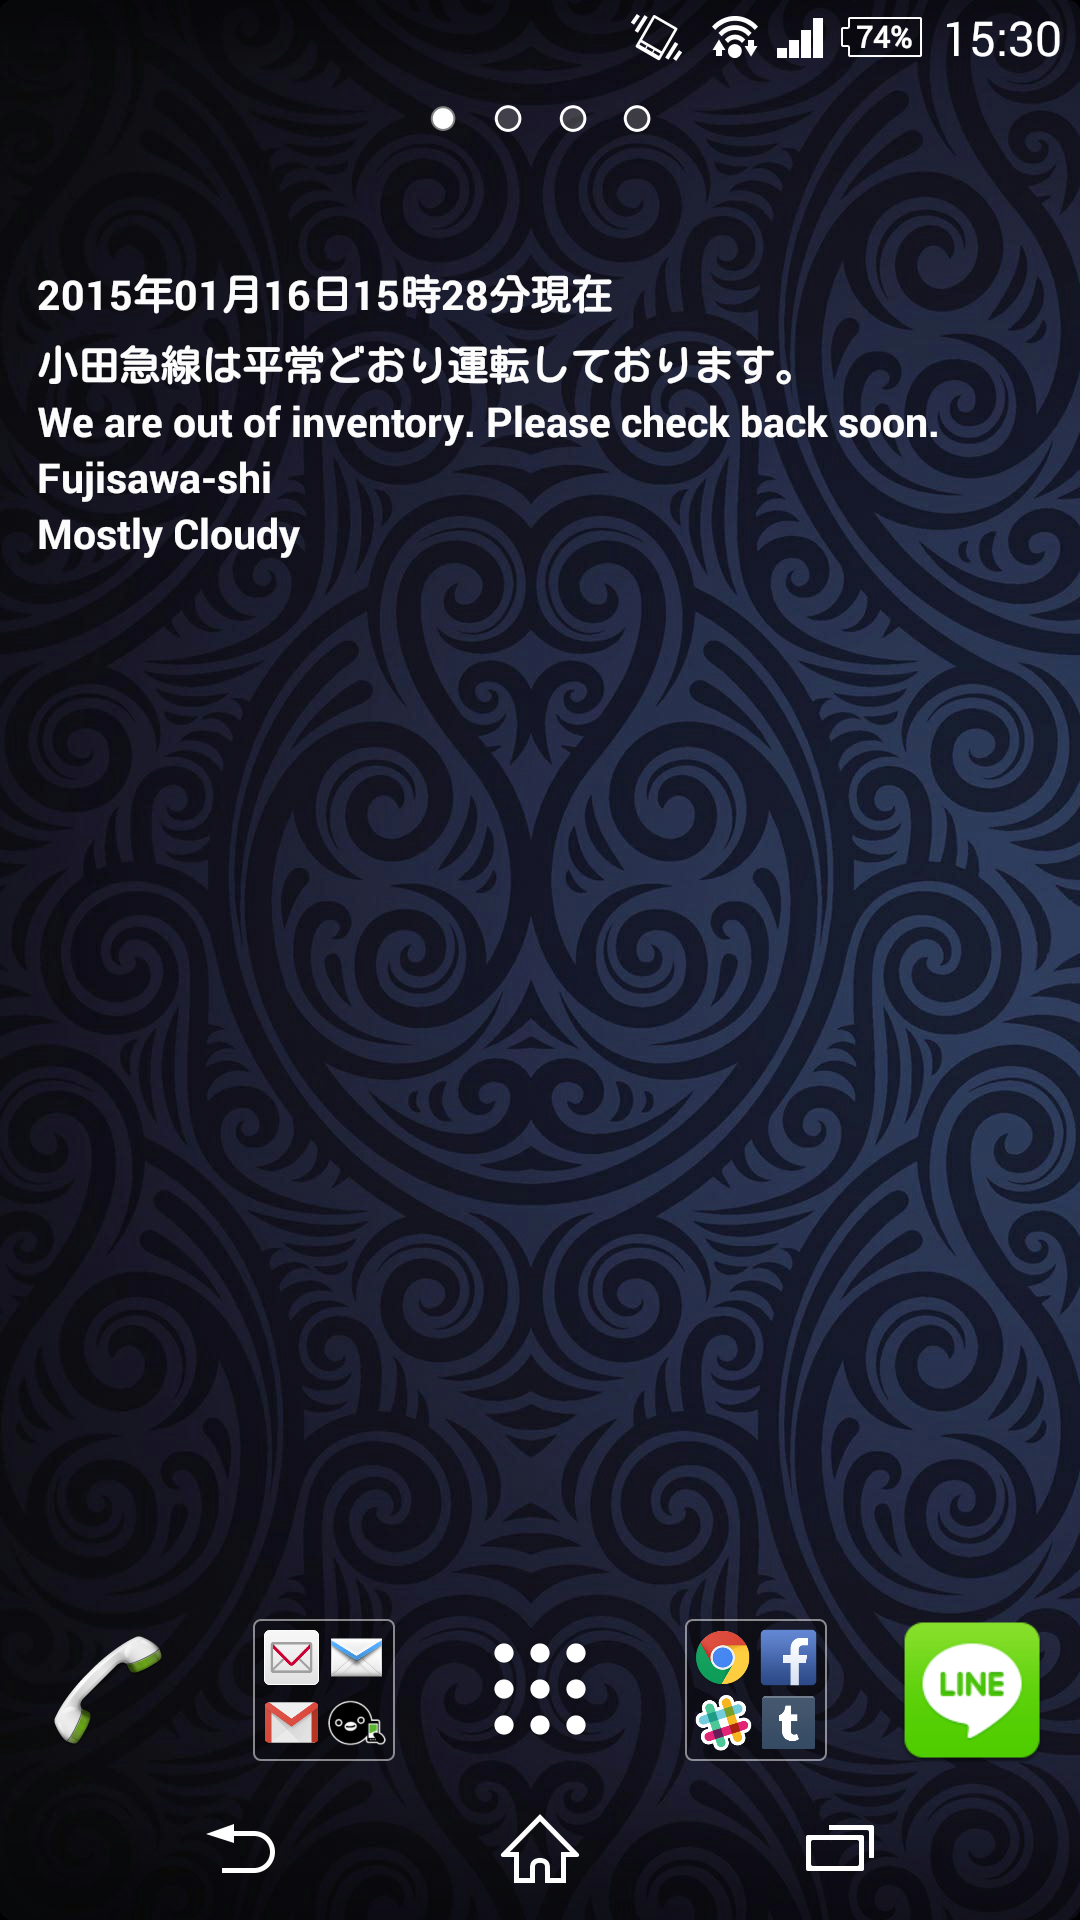
\includegraphics[width=100mm]{image/widget_single.eps}}
    \end{center}
    \caption{Android Widgetとして表示する例}
    \label{fig:widget}
  \end{minipage}
\end{figure}

\nocite{*}
  % 本文2
\chapter{実装}
\label{chap:prototype}

この章では本研究でのプロトタイプを実装し、その流れを解説する。

\section{実装概要}
実装に際してサーバーサイドはNode.js\footnote{https://nodejs.org/}を用いて実装した。またデータベースにはmongoDB\footnote{http://www.mongodb.org/}を採用している。

AndroidクライアントサイドにはJava\footnote{https://java.com/}を用いた。

\subsection{サーバーサイド}
言語はJavascriptを使い、Node.jsのsocket.ioで実装した。
以下のことを書く。

- Lindaとのデータのやりとり(socket.io)

- 同期処理(async)

- DBに存在する数だけ繰り返し(underscore.jsのeach)

\subsection{Androidサイド}
Androidクライアントサイドの実装にはJavaを用いた。
以下のことを書く。

- 表示内容の更新のための操作

- サーバーへのリクエストに用いた技術(Volley)

- JSONのパースに用いた技術(JSONObject)
  % 本文3
\chapter{考察}
\label{chap:consideration}

\section{本研究についての考察}
A 「結果」(調査や分析の結果)を解釈して「目的」で述べられた研究課題への回答となる諸命題を引き出す。
(結論として何が分かったのかを示す。このAが「考察」の中核部分である。)

B かかる命題の成立条件や限定範囲があれば但し書きをつける。(命題とその付帯条件が結論となる)

C 「対象と方法」で記述した、調査や分析の手続きについて弱点ないし誤解を生じやすい点があれば、補足説明をする。

D 自ら提起する新たな知見と先行研究との関係に言及する。
問題は解決できたのか。
自分で使ってどう感じたのかを書く。(成功だったのかどうか)

現在、インターネット上には様々な情報が溢れている。それだけでなく個人が自ら情報を発信することも容易になっている。

作成したシステムを実際に使用して気づいた点
問題の解決に成功した点
不要な情報が表示されない
情報の取捨選択が容易

問題点
- テキストデータしかとれないが、取りたい情報がテキストデータとは限らない。
- 見やすさを考えた時に、現状がベストとは言えない。
  % 本文4
\chapter{結論}
\label{chap:conclusion}

本研究では、ユーザーが必要とする複数の情報を表示するシステム及びインターフェースの実現を試みた。結果として必要な情報に付随して不必要な情報が表示される問題や、多くのAndroid Widgetを置くことで画面スペースを占有してしまう問題、自分の取得したい情報に対応するAndroid Widgetが存在しない場合、自らAndroid Widgetを作成するしか対応策が無い、といった問題を解決することができた。

そして、第\ref{chap:consideration}章で述べたようにいくつかの課題が見つかった。さらに効率のよい情報の獲得を目指し、これらの課題の解決に今後も取り組んでいきたい。
  % 本文5

\begin{acknowledgment}

\begin{flushright}
中山 拓哉
\end{flushright}

\end{acknowledgment}
  % 謝辞。要独自コマンド、include先参照のこと

\begin{bib}[100]
% BibTeXを使う場合
\bibliography{main}

%\begin{thebibliography}{#1}
%
%  \bibitem{参照用名称}
%    著者名:
%    \newblock 文献名,
%    \newblock 書誌情報,出版年.
%
% \bibitem{hoge09}
%   ほげ山太郎,ほげ山次郎:
%   \newblock ほげほげ理論のHCI分野への応用,
%   \newblock ほげほげ学会論文誌,Vol.31,No.3,pp.194-201,2009.
%
% \bibitem{hoge08}
%   Taro Hogeyama, Jiro Hogeyama:
%   \newblock The Theory of Hoge,
%   \newblock {\it The Proceedings of The Hoge Society}, 2008.
%
%\end{thebibliography}

\end{bib}
  % 参考文献。要独自コマンド、include先参照のこと
\appendix
%\chapter{付録の例}

付録を無理矢理出力させるため、てきとうなことを書く。

\section{ほげ}

コマンドは本文と一緒。

\subsection{ふー}

本文と一緒。

\section{ほげほげ}

本文と一緒。

\subsection{ふーふー}

本文と一緒。
    % 付録

\end{document}
